%========================================================================================
%  PRESENTAZIONE DI LAUREA — Lorenzo Caivano
%  File principale: compila SEMPRE questo file (VS Code + LaTeX Workshop).
%  Le slide stanno nei file della cartella Slide/ — qui ci sono solo impostazioni
%  e l'elenco delle slide.
%  Le figure sono prese direttamente da ../Tesi_LaTeX/Figure (nessuna copia):
%  il PDF finale le contiene già, quindi sulla chiavetta basta main.pdf.
%========================================================================================

\documentclass[aspectratio=169, 11pt]{beamer}
% aspectratio=169 -> formato 16:9  (per 4:3 togli l'opzione)

\usepackage[utf8]{inputenc}
\usepackage[T1]{fontenc}
\usepackage[italian]{babel}
\usepackage{lmodern}          % font vettoriali, inclusi nel PDF
\usepackage{amsmath, amssymb}
\usepackage{graphicx}
\usepackage{booktabs}         % tabelle con \toprule, \midrule, \bottomrule
\usepackage{appendixnumberbeamer} % le slide di riserva non contano nel totale

% Cartella delle figure: si usano quelle della tesi, senza copiarle
\graphicspath{{../Tesi_LaTeX/}}

%----------------------------------------------------------------------------------------
%	COLORI (gli stessi delle figure della tesi)
%----------------------------------------------------------------------------------------
\definecolor{reali}{HTML}{2E86AB}      % dati reali (blu)
\definecolor{simul}{HTML}{F4A261}      % simulazioni (arancione)
\definecolor{simdue}{HTML}{6A4C93}     % seconda simulazione (viola)
\definecolor{enterprise}{HTML}{C73E1D} % Enterprise / DR2new+ (rosso)
\definecolor{grigio}{HTML}{555555}

%----------------------------------------------------------------------------------------
%	TEMA: semplice, senza fronzoli
%----------------------------------------------------------------------------------------
\usetheme{default}
\setbeamertemplate{navigation symbols}{}            % niente icone di navigazione
\setbeamercolor{frametitle}{fg=reali}
\setbeamercolor{title}{fg=reali}
\setbeamercolor{structure}{fg=reali}
\setbeamercolor{normal text}{fg=black}
\setbeamerfont{frametitle}{size=\Large, series=\bfseries}
\setbeamertemplate{itemize items}[circle]
\setbeamertemplate{footline}{%
  \hfill{\color{grigio}\scriptsize\insertframenumber\,/\,\inserttotalframenumber}\hspace{4mm}\vspace{3mm}}

%----------------------------------------------------------------------------------------
%	SCORCIATOIE (come nella tesi)
%----------------------------------------------------------------------------------------
\newcommand{\Agwb}{A_{\mathrm{GWB}}}
\newcommand{\gammagwb}{\gamma_{\mathrm{GWB}}}
\newcommand{\fyr}{f_{\mathrm{yr}}}
\newcommand{\reali}[1]{\textcolor{reali}{#1}}
\newcommand{\simul}[1]{\textcolor{simul}{#1}}

% Ritagli dei corner plot a 6 parametri (figure 8x8 pollici, ordine dei parametri:
% gamma_DM, logA_DM, gamma_RN, logA_RN, gamma_SV, logA_SV).
% trim = sinistra basso destra alto (in pt). Se un ritaglio non ti convince, cambia
% questi numeri: valgono per tutte le slide.
%   \cornerDMSV : blocco 2x2 in basso a sinistra (DM contro scattering)
%   \cornerDM   : blocco 2x2 in alto a sinistra (istogramma di gamma_DM e piano A_DM-gamma_DM)
\newcommand{\cornerDMSV}[2][height=0.75\textheight]{%
  \includegraphics[#1, trim=0 0 362 348, clip]{#2}}
\newcommand{\cornerDM}[2][height=0.75\textheight]{%
  \includegraphics[#1, trim=0 396 362 0, clip]{#2}}

%----------------------------------------------------------------------------------------
%	TITOLO
%----------------------------------------------------------------------------------------
\title{Studio delle degenerazioni\\nell'analisi del rumore delle pulsar}
\author{Lorenzo Caivano}
\institute{Università degli Studi di Milano-Bicocca\\
           Corso di Laurea in Fisica}
\date{Relatore: Prof.\ Alberto Sesana \quad Correlatrice: Dott.ssa Irene Ferranti}

%========================================================================================
\begin{document}

% !TEX root = ../main.tex
%--- Slide 1: titolo (circa 15 s) -------------------------------------------------------
\begin{frame}[plain]
  \centering
  
\includegraphics[height=2.2cm]{Figure/logo.png}\par\vspace{6mm}
  {\usebeamercolor[fg]{title}\LARGE\bfseries Studio delle degenerazioni\\[1mm]
   nell'analisi del rumore delle pulsar\par}
  \vspace{2mm}
  {\small\color{grigio}\itshape Study of degeneracies in pulsar noise analysis\par}
  \vspace{8mm}
  {\large Lorenzo Caivano\par}
  \vspace{5mm}
  {\small Relatore: Prof.\ Alberto Sesana \qquad Correlatrice: Dott.ssa Irene Ferranti\par}
  \vspace{4mm}
  {\small Corso di Laurea in Fisica\par}
\end{frame}

% !TEX root = ../main.tex
%--- Slide 2: pulsar timing array (circa 1 min) ------------------------------------------
% Figure: Figure/P02_hellings_downs.pdf e Figure/P02_power_law.pdf (notebook 28).
\begin{frame}{Pulsar timing array}
  \small
  \begin{itemize}\setlength{\itemsep}{1pt}
    \item \textbf{Millisecond pulsar} (MSP): impulsi radio regolari come orologi atomici
    \item Un'onda gravitazionale tra la Terra e la pulsar fa arrivare gli impulsi
          in anticipo o in ritardo
    \item \textbf{Pulsar timing array}: si misurano per anni i tempi di arrivo (TOA) di molte pulsar,
          quindi si osservano onde a frequenze dei nHz
    \item Il fondo stocastico (\textbf{GWB}) è un segnale comune, \textbf{correlato tra le pulsar}
          (curva di Hellings--Downs). Prime evidenze nel 2023
    \item È un \textbf{processo stocastico} con spettro a \textbf{legge di potenza},
          $S(f) \propto A^2 (f/\fyr)^{-\gamma}$, come i rumori della pulsar
  \end{itemize}
  \vspace{1mm}
  \centering
  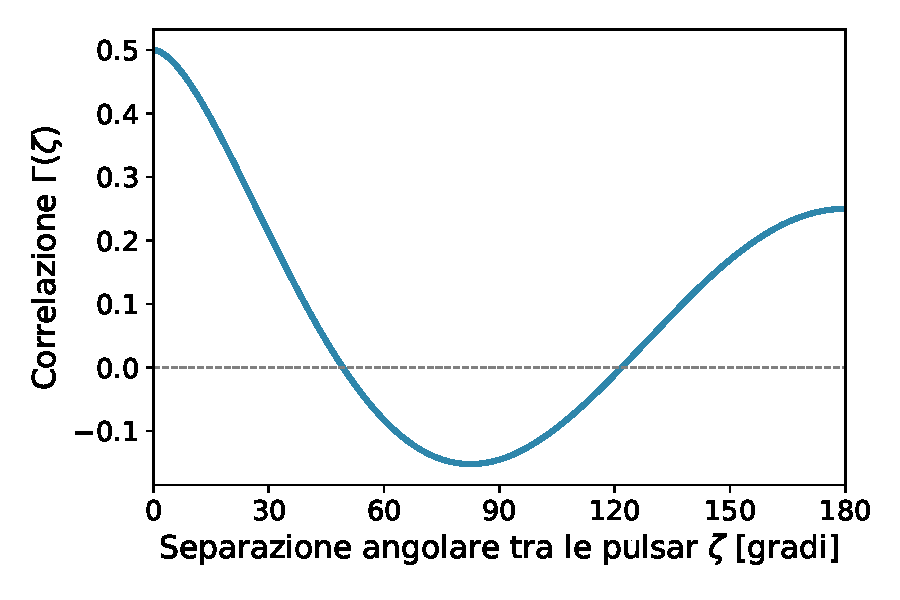
\includegraphics[height=0.38\textheight]{Figure/P02_hellings_downs.pdf}\hfill
  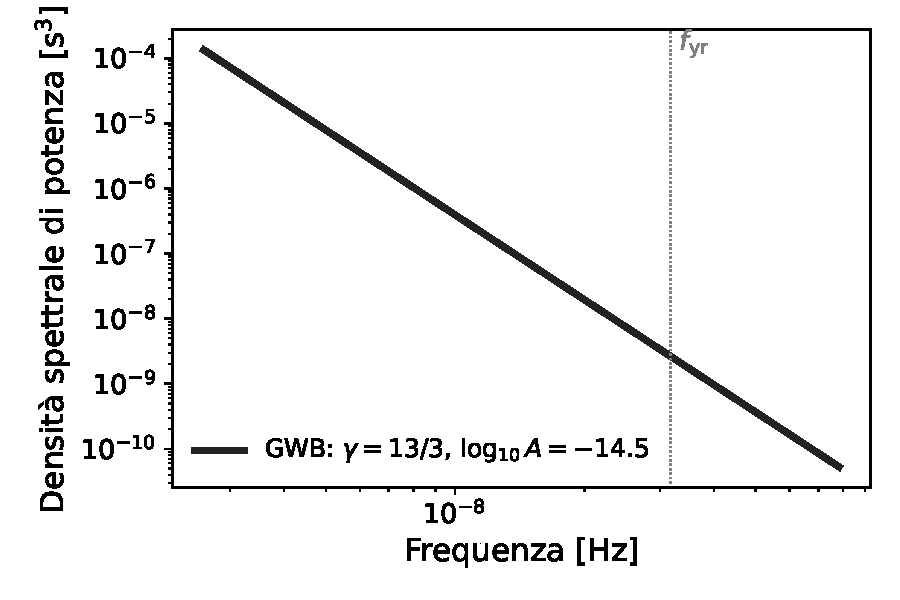
\includegraphics[height=0.38\textheight]{Figure/P02_power_law.pdf}
\end{frame}

% !TEX root = ../main.tex
%--- Slide 3: il modello di rumore (circa 1 min 15 s) ------------------------------------
\begin{frame}{Il modello di rumore}
  \small
  \begin{itemize}\setlength{\itemsep}{2pt}
    \item \textbf{White noise}: errori di misura indipendenti da un TOA all'altro (fissato)
    \item \textbf{Rumori rossi}: processi stocastici a legge di potenza come il GWB ($A$, $\gamma$):
          potenza alle basse frequenze, cioè variazioni lente, su scale di anni
  \end{itemize}
  \vspace{2mm}
  \centering
  \renewcommand{\arraystretch}{1.1}
  \begin{tabular}{lllc}
    \toprule
    Processo & Origine & Tipo & Ritardo $\propto$ \\
    \midrule
    GWB                       & onde gravitazionali   & acromatico & $\nu^{0}$ \\
    Red noise intrinseco (RN) & rotazione della pulsar & acromatico & $\nu^{0}$ \\
    Variazioni di DM          & elettroni liberi & \textbf{cromatico} & $\nu^{-2}$ \\
    Variazioni di scattering (SV) & mezzo interstellare & \textbf{cromatico} & $\nu^{-4}$ \\
    \bottomrule
  \end{tabular}
  \vspace{2mm}
  \begin{itemize}\setlength{\itemsep}{2pt}
    \item \textbf{Cromatico}: il ritardo cresce a bassa frequenza radio $\nu$:
          per separarli servono osservazioni a più frequenze
    \item GWB e RN hanno la stessa firma acromatica: in una singola pulsar non si distinguono
    \item Modello di riferimento: RN + DM + SV, \textbf{6 parametri liberi}
  \end{itemize}
\end{frame}

% !TEX root = ../main.tex
%--- Slide 4: i residui di J1640+2224 (circa 50 s) --------------------------------------
\begin{frame}{I residui di timing di PSR J1640+2224}
  \centering
  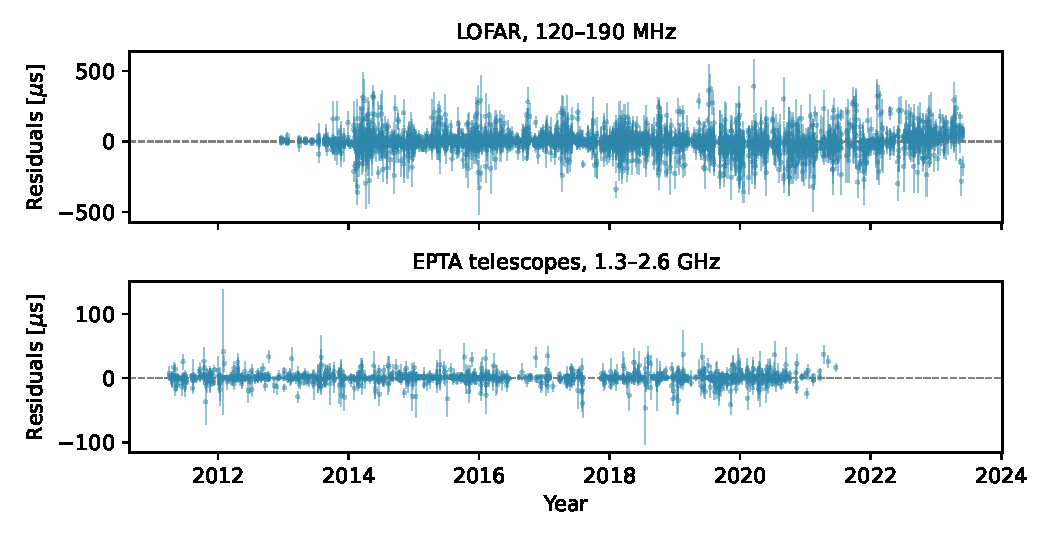
\includegraphics[width=0.78\textwidth]{Figure/cap2/residuals_J1640.pdf}\par
  \vspace{2mm}
  \begin{itemize}
    \item Residui = TOA osservati $-$ TOA previsti dal modello di timing
    \item Dataset \textbf{DR2low}: EPTA DR2new+ (1.3--2.6\,GHz) + LOFAR (120--190\,MHz)
    \item I TOA di LOFAR hanno incertezze molto più grandi
  \end{itemize}
\end{frame}

% !TEX root = ../main.tex
%--- Slide 5: metodo e ruolo di LOFAR (circa 50 s) ---------------------------------------
\begin{frame}{Metodo e ruolo delle basse frequenze}
  \begin{columns}[c]
    \column{0.45\textwidth}
    \begin{itemize}
      \item Inferenza bayesiana, campionamento MCMC
      \item Codice Discovery: likelihood compilata con JAX, validato con Enterprise (stesse posterior sugli stessi dati)
      \item Confronto \reali{DR2low} e \textcolor{enterprise}{DR2new+}\\
          
      \item Senza LOFAR il rumore cromatico\\ non è vincolato:
            le posterior riempiono il prior
    \end{itemize}
    \column{0.52\textwidth}
    \centering
    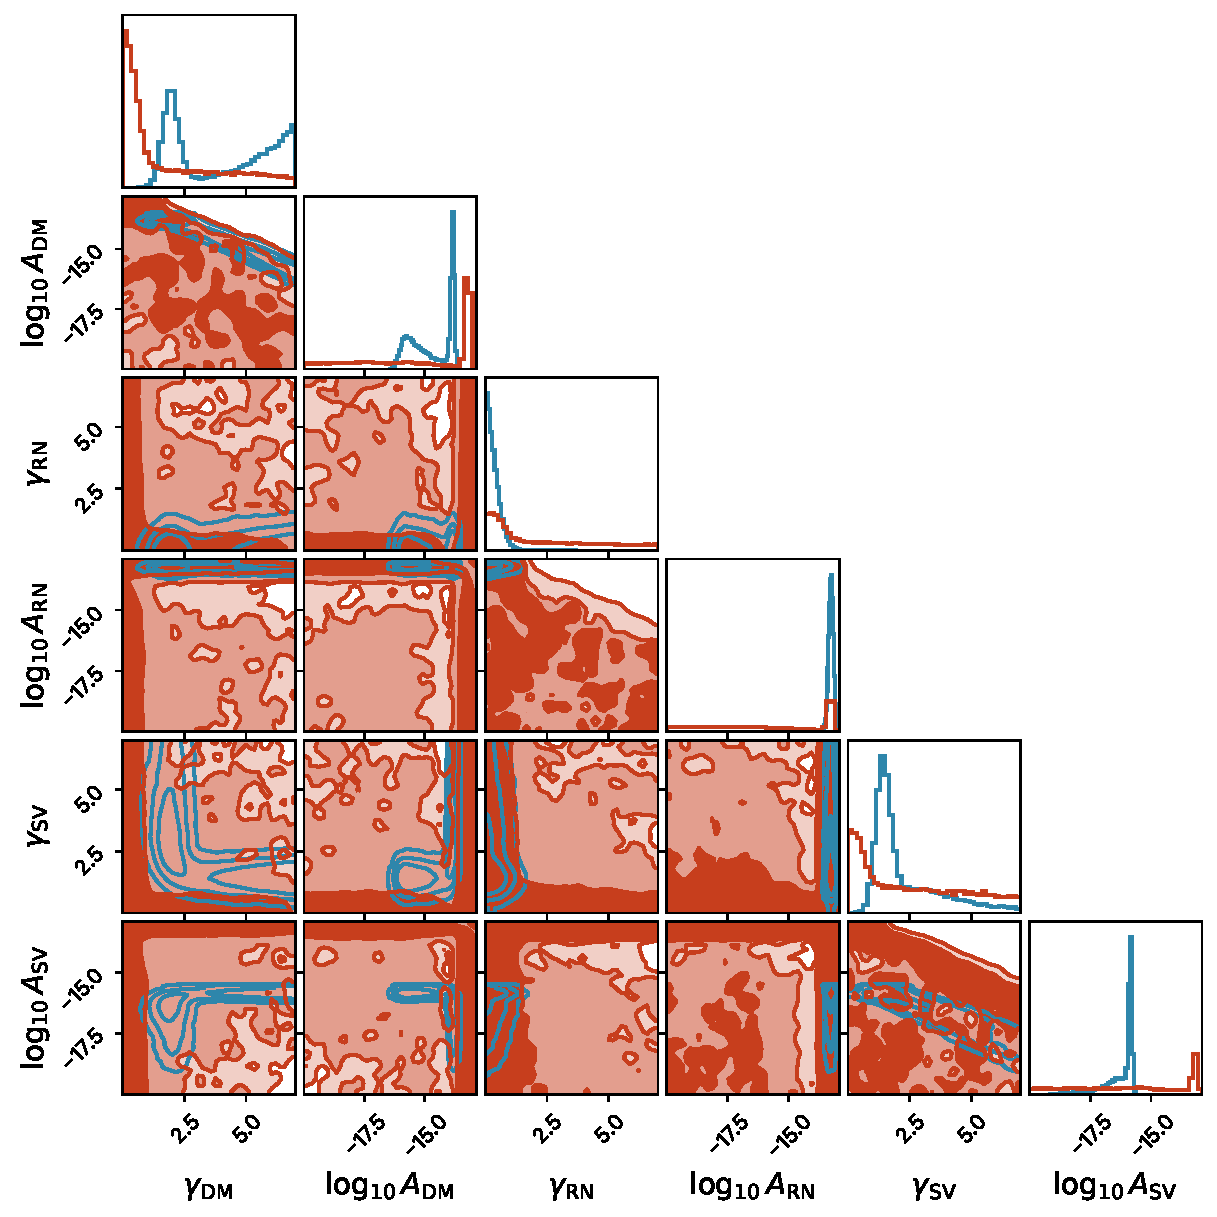
\includegraphics[height=0.8\textheight]{Figure/cap5/02_DR2low_vs_DR2newplus.pdf}
  \end{columns}
\end{frame}

% !TEX root = ../main.tex
%--- Slide 6: la degenerazione DM-scattering (circa 1 min 15 s) --------------------------
% Figura: Figure/P06_reali_DM_SV.pdf (notebook 26), solo dati reali DR2low.
\begin{frame}{La degenerazione DM--scattering}
  \begin{columns}[c]
    \column{0.45\textwidth}
    \centering
    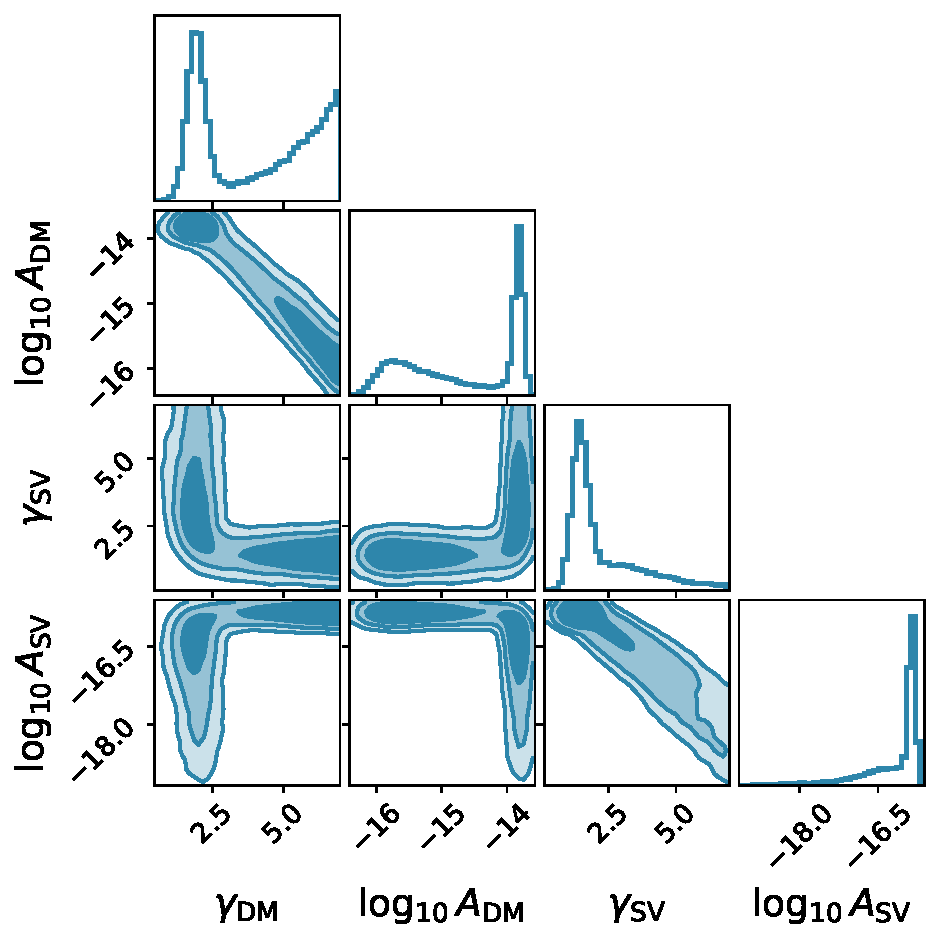
\includegraphics[height=0.82\textheight]{Figure/P06_reali_DM_SV.pdf}
    \column{0.52\textwidth}
    \begin{itemize}
      \item Il DM ha \textbf{due picchi}:
        \begin{itemize}
          \item ampiezza alta: $\log_{10}A_{\rm DM} \simeq -13.8$, $\gamma_{\rm DM} \simeq 2$
          \item ampiezza bassa: $\log_{10}A_{\rm DM} \simeq -15.5$, $\gamma_{\rm DM}$ al bordo del prior
        \end{itemize}
      \item Tra DM e scattering i contorni hanno \textbf{forma a L}
      \item Il rumore cromatico si descrive con il DM \emph{o} con lo scattering:
            i dati non scelgono
    \end{itemize}
  \end{columns}
\end{frame}

% !TEX root = ../main.tex
%--- Slide 7: la degenerazione non dipende dal modello (circa 50 s) ----------------------
% Figura: Figure/P07_reali_8par_BN_DM.pdf (notebook 26) = Fig. 5.3 della tesi ridotta a band noise e DM.
\begin{frame}{La degenerazione resta con modelli più complessi}
  \begin{columns}[c]
    \column{0.52\textwidth}\small
    \textbf{Band noise nel modello} (8 parametri)
    \begin{itemize}\setlength{\itemsep}{1pt}
      \item Rumore rosso solo sui TOA della banda LOFAR
      \item Non rivelato: solo un limite superiore
            $\log_{10}A_{\rm BN} < -12.21$ (95\%)
      \item Il DM ha ancora due picchi
    \end{itemize}
    \vspace{2mm}
    \textbf{Indice cromatico $\alpha$ libero} (7 parametri)
    \begin{itemize}\setlength{\itemsep}{1pt}
      \item $\alpha = 3.31^{+0.60}_{-0.46}$
      \item Due picchi e contorni a L restano
    \end{itemize}
    \vspace{3mm}
    \fbox{\parbox{0.92\linewidth}{\centering
      La degenerazione non è dovuta a un modello impreciso dello scattering}}
    \column{0.46\textwidth}
    \centering
    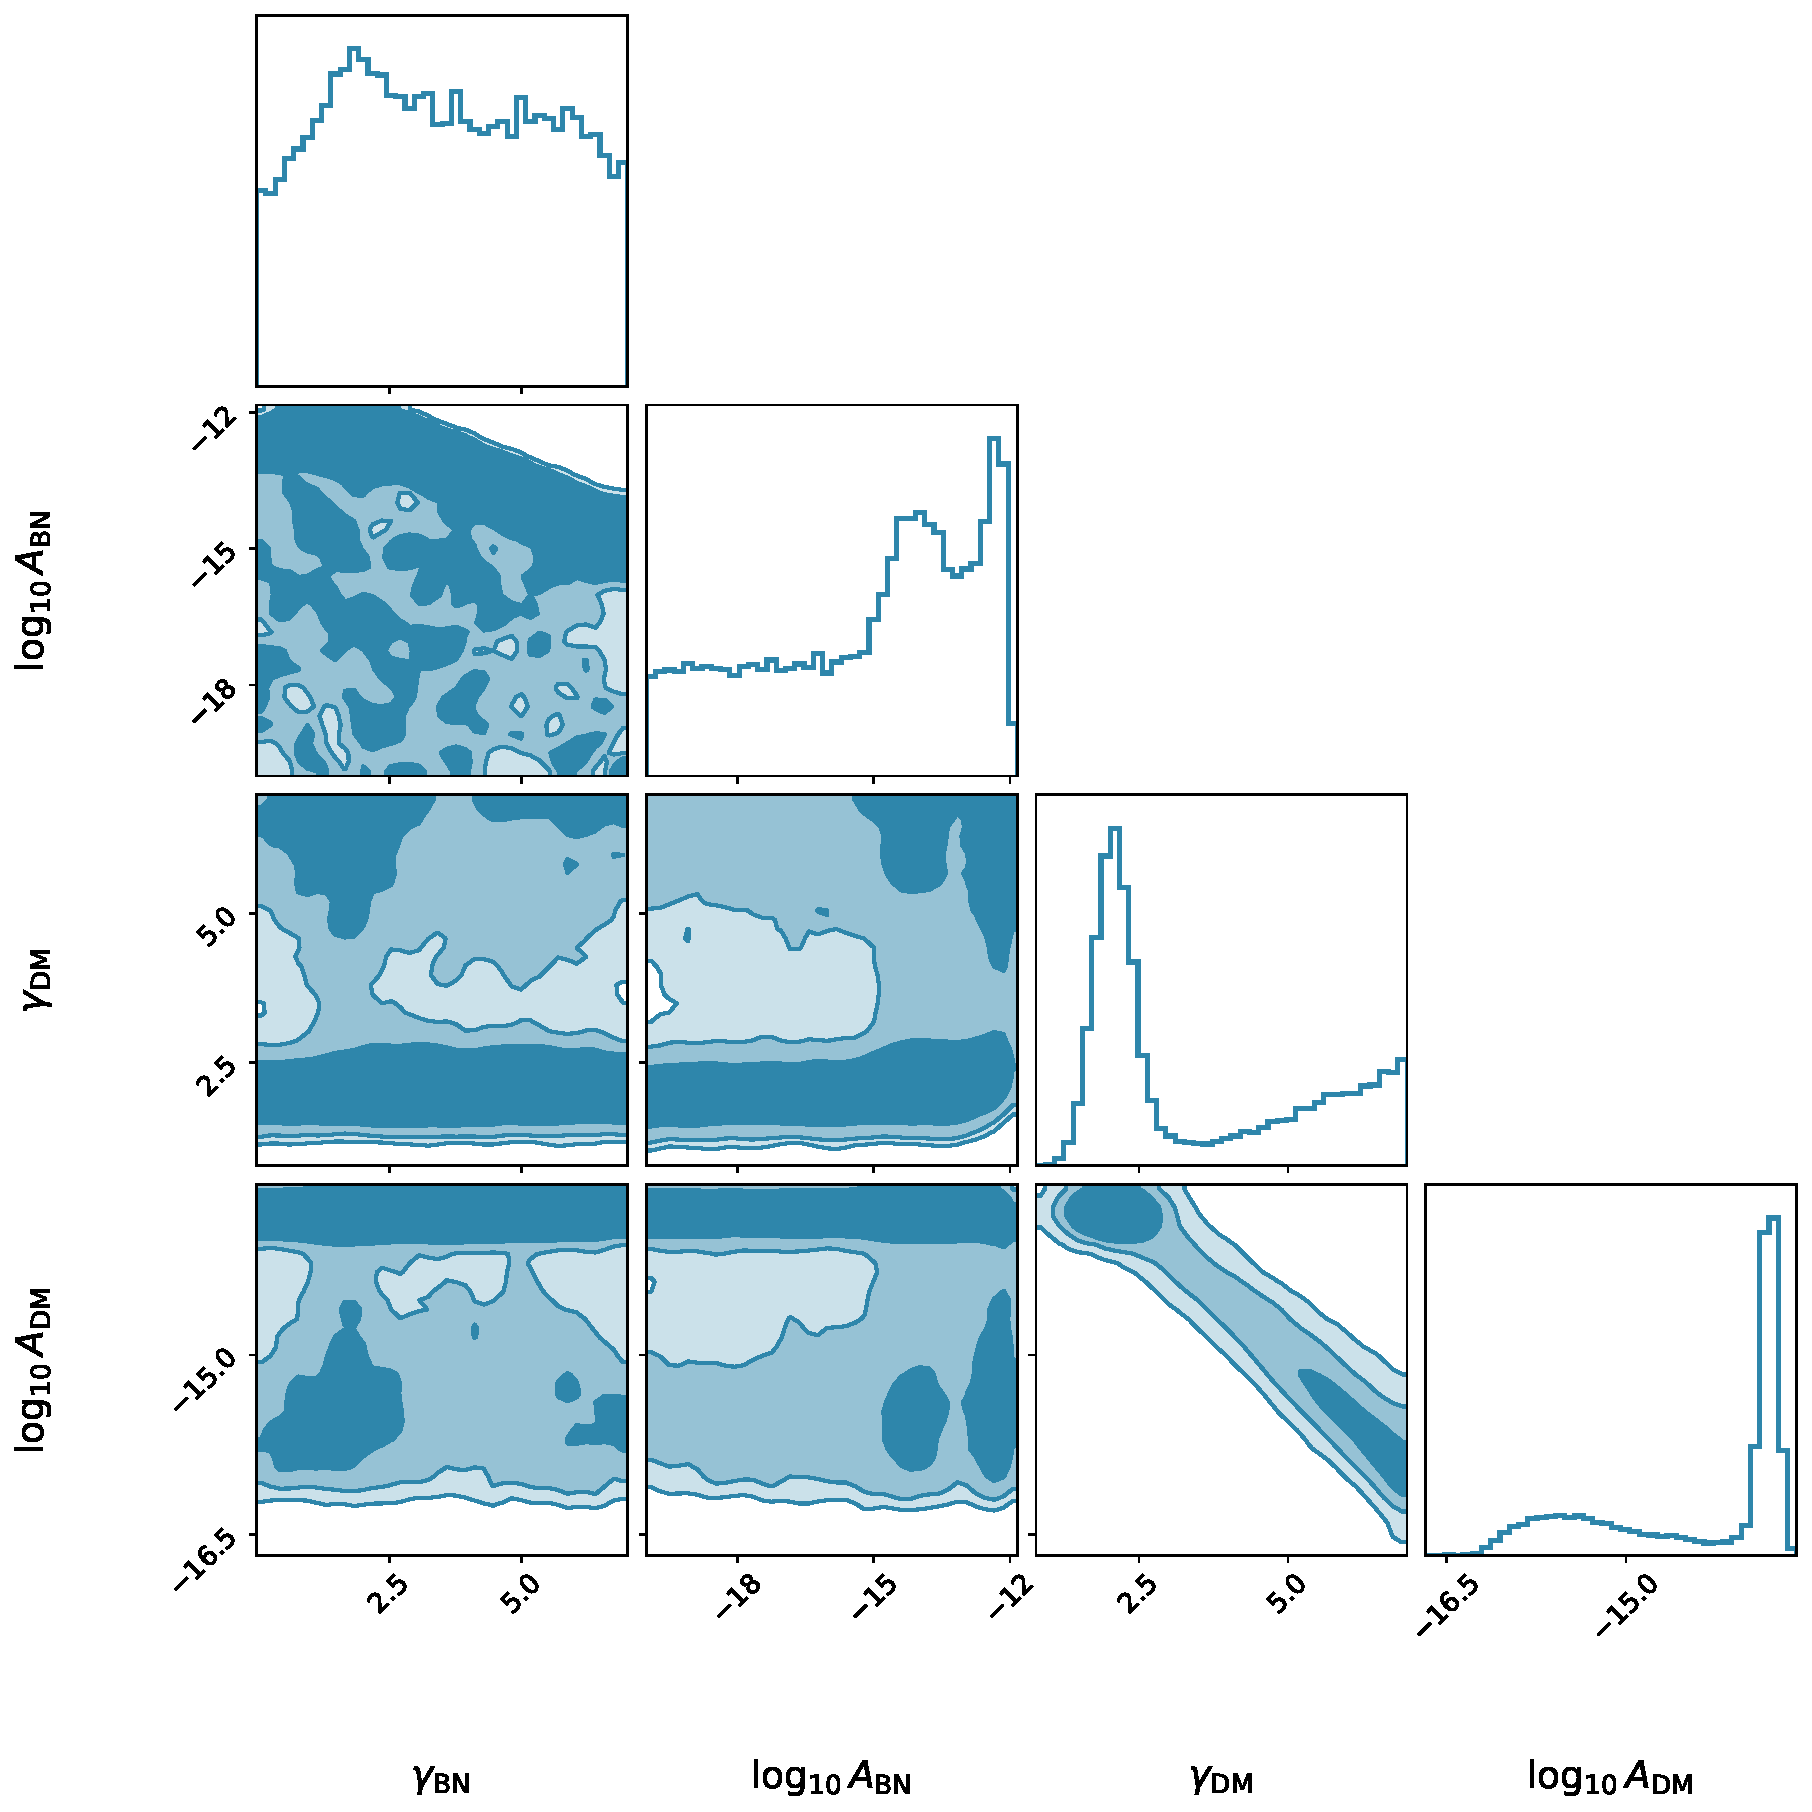
\includegraphics[height=0.72\textheight]{Figure/P07_reali_8par_BN_DM.pdf}\par
    {\footnotesize \reali{dati reali}, modello con band noise}
  \end{columns}
\end{frame}

% !TEX root = ../main.tex
%--- Slide 8: simulazione di riferimento (circa 50 s) ------------------------------------
\begin{frame}{Simulazione di riferimento}
  \begin{columns}[c]
    \column{0.55\textwidth}
    \begin{itemize}
      \item Stessi TOA, incertezze e frequenze di DR2low
      \item Residui sostituiti da una realizzazione dei soli tre processi del modello
      \item \simul{Simulazione}: parametri iniettati recuperati,\\
            un solo picco, niente L
      \item La copertura in frequenza di DR2low basta a distinguere DM e scattering
    \end{itemize}
    \column{0.42\textwidth}
    \centering
    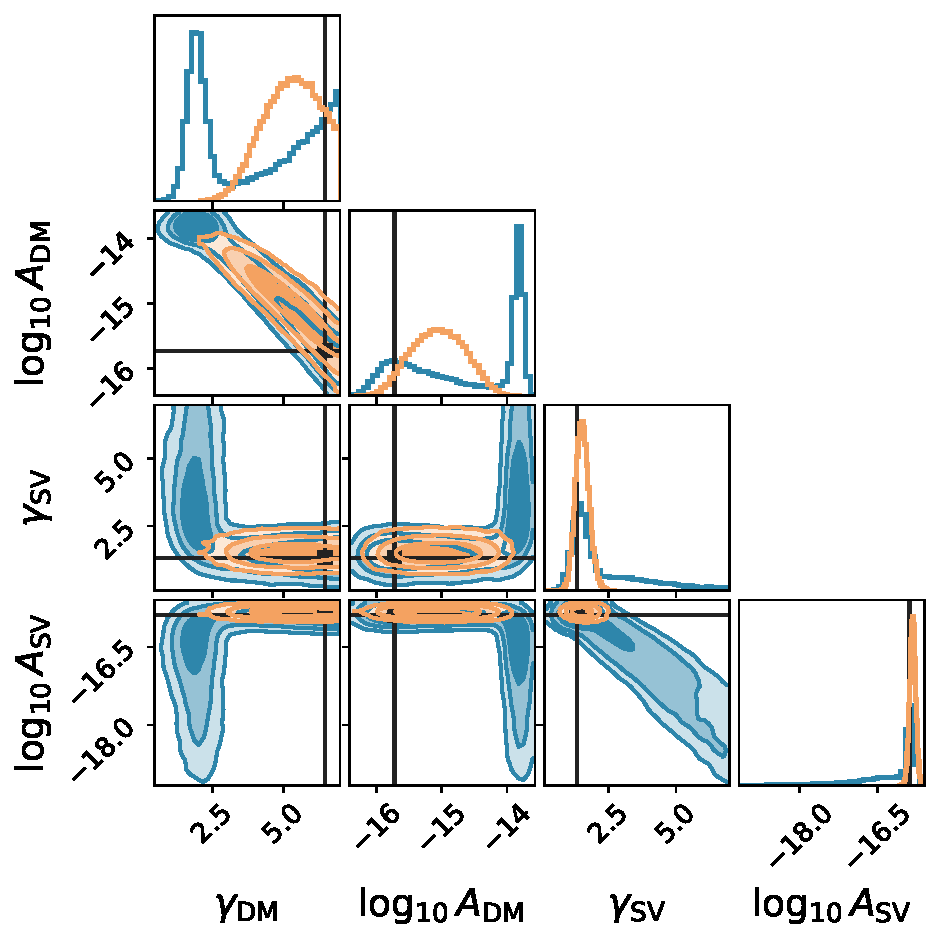
\includegraphics[height=0.72\textheight]{Figure/P08_reali_vs_sim_DM_SV.pdf}\par
    {\footnotesize \reali{dati reali} \quad \simul{simulazione}\\ linee nere: valori iniettati}
  \end{columns}
\end{frame}

% !TEX root = ../main.tex
%--- Slide 9: processi non modellati (circa 1 min 45 s) -----------------------------------
% Una sola slide ripetuta 3 volte (overlay 1, 2, 3): cambia il caso evidenziato e la figura.
% Figure: Figure/P09_1_GWB.pdf, P09_2_band.pdf, P09_3_GWB_band.pdf (notebook 26).
% Colori: dati reali blu, simulazione di riferimento arancione, nuova simulazione viola.
\begin{frame}{Processi presenti nei dati ma non nel modello}
  \setbeamercovered{transparent=25}
  \begin{columns}[c]
    \column{0.53\textwidth}\small
    Simulazioni con un processo in più, analizzate con il modello a 6 parametri
    \vspace{0.5mm}

    \uncover<1>{%
    \textbf{GWB} ($\log_{10}\Agwb$ da $-15.5$ a $-14.5$)
    \begin{itemize}\setlength{\itemsep}{0pt}
      \item Il red noise intrinseco cambia poco
      \item Deboli code a L, solo nei contorni al 99.7\%
    \end{itemize}}
    \vspace{0.5mm}

    \uncover<2>{%
    \textbf{Band noise} ($\log_{10}A_{\rm BN} = -12.5$)
    \begin{itemize}\setlength{\itemsep}{0pt}
      \item DM verso ampiezza alta e indice basso: zona del picco alto dei dati reali
      \item Ma un solo picco, niente L
    \end{itemize}}
    \vspace{0.5mm}

    \uncover<3>{%
    \textbf{GWB + band noise} ($-14$ e $-12.5$)
    \begin{itemize}\setlength{\itemsep}{0pt}
      \item DM spostato come con il solo band noise; red noise più forte e ripido
      \item Ma un solo picco, niente L
    \end{itemize}}
    \column{0.45\textwidth}
    \centering
    \only<1>{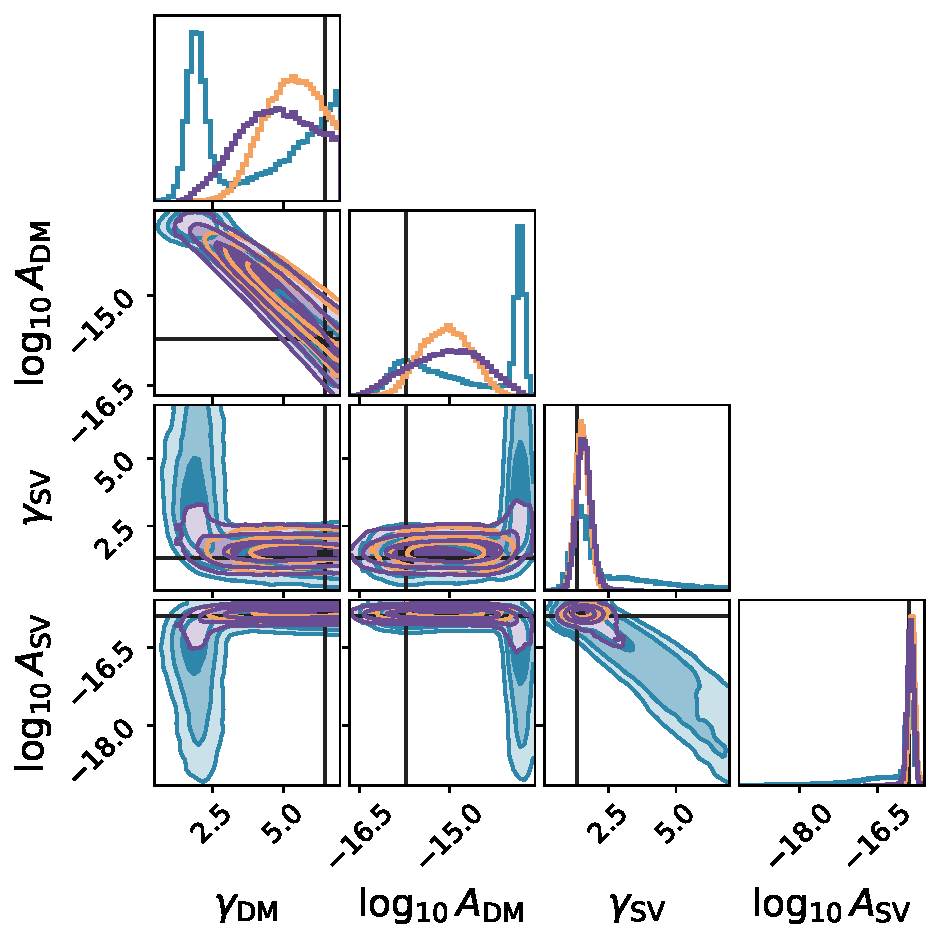
\includegraphics[height=0.66\textheight]{Figure/P09_1_GWB.pdf}}%
    \only<2>{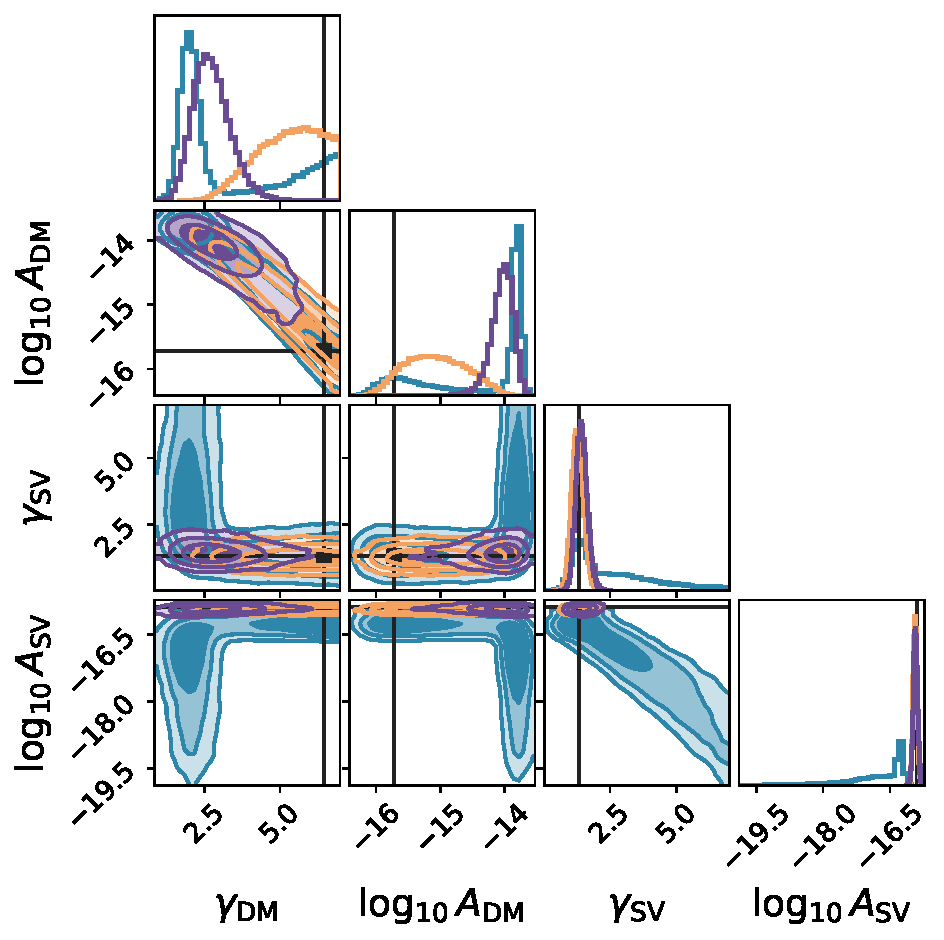
\includegraphics[height=0.66\textheight]{Figure/P09_2_band.pdf}}%
    \only<3>{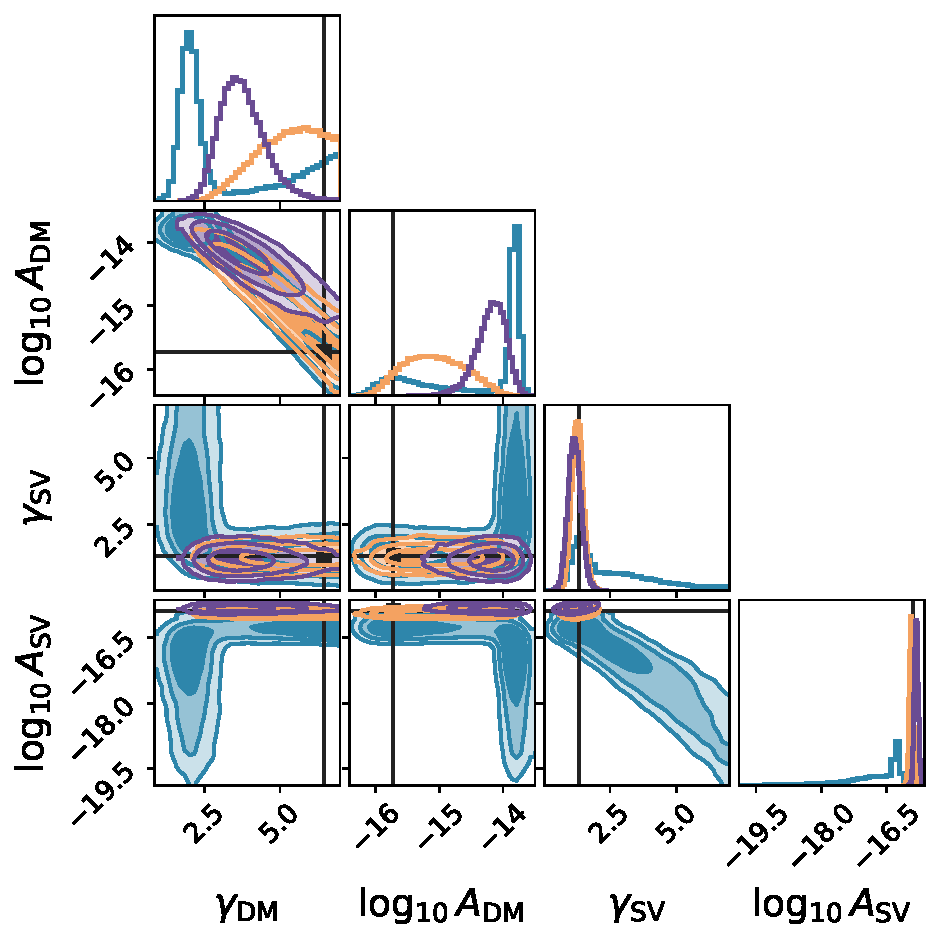
\includegraphics[height=0.66\textheight]{Figure/P09_3_GWB_band.pdf}}\par
    {\footnotesize \reali{dati reali} \quad \simul{riferimento} \quad
     \textcolor{simdue}{nuova simulazione}\\
     linee nere: valori iniettati}
  \end{columns}
\end{frame}

% !TEX root = ../main.tex
%--- Slide 10: un band noise che non si vede (circa 50 s) --------------------------------
% Figura: Figure/P11_logA_BN_due_pannelli.pdf (notebook 26): posterior di log10 A_BN,
% dati reali (blu) vs simulazione (viola) iniettata a -12.5 e a -12, modello a 8 parametri.
\begin{frame}{Un band noise che non si vede}
  \small
  \textcolor{simdue}{Simulazioni} analizzate con il band noise nel modello (8 parametri)
  \begin{itemize}\setlength{\itemsep}{1pt}
    \item Il band noise resta non rivelato fino a $-12.5$ ($\log_{10}A_{\rm BN} < -12.36$ al 95\%)
          e viene rivelato solo a $-12$, perché i TOA di LOFAR hanno grandi incertezze
    \item \reali{Dati reali}: $\log_{10}A_{\rm BN} < -12.21$ (95\%), simile alla simulazione con $-12.5$
    \item Un band noise non rivelato può indurre un bias nel DM
    \item \textbf{Non può essere esclusa la presenza di un band noise nei dati reali}
  \end{itemize}
  \vspace{1mm}
  \centering
  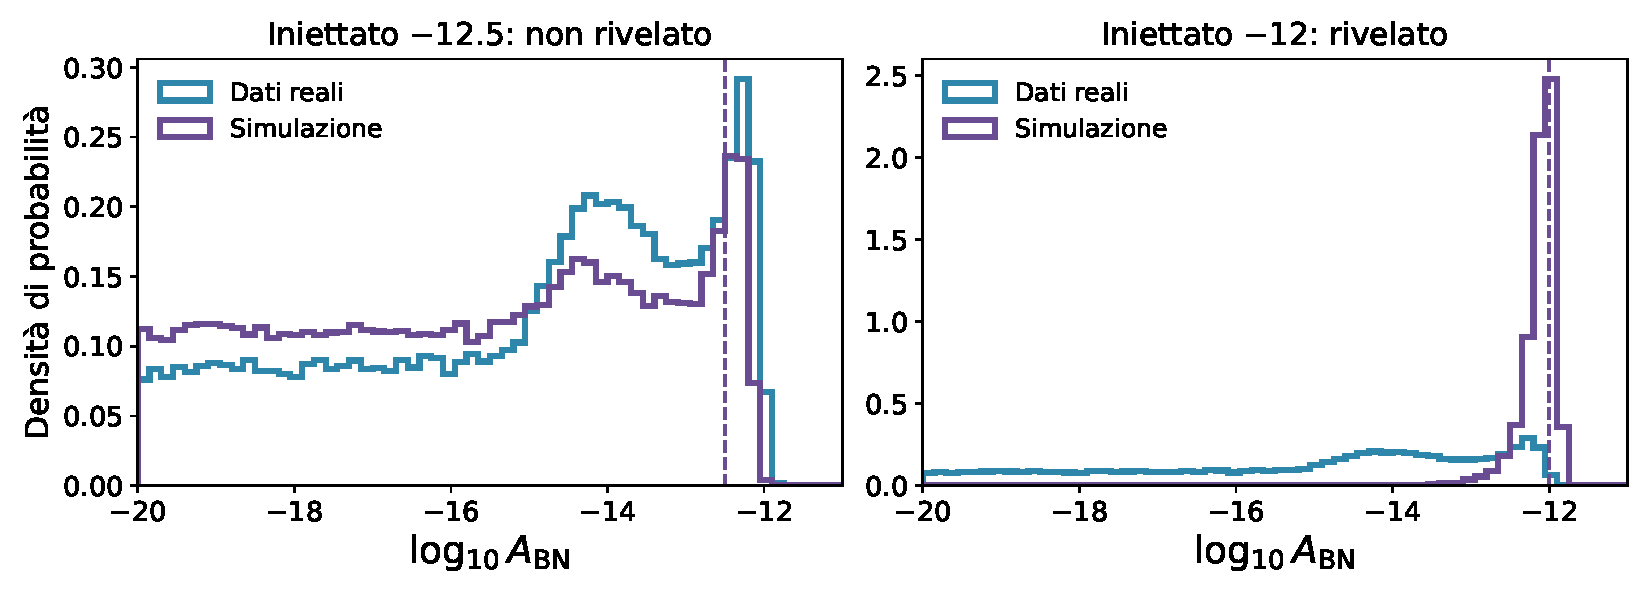
\includegraphics[width=0.80\textwidth]{Figure/P11_logA_BN_due_pannelli.pdf}
\end{frame}

% !TEX root = ../main.tex
%--- Slide 11: conclusioni (circa 1 min) --------------------------------------------------
\begin{frame}{Conclusioni}
  \begin{itemize}\setlength{\itemsep}{3pt}
    \item Nei dati reali DM e scattering sono \textbf{degeneri} (due picchi, forma a L);
          nelle simulazioni senza processi non modellati no
    \item \textbf{GWB} non modellato: solo deboli code a L
    \item \textbf{Band noise} non modellato: sposta il DM e ne riproduce il picco ad alta ampiezza
          dei dati reali, ma non la forma a L
    \item Un band noise può indurre un bias nel DM senza essere rivelato:
          \textbf{non può essere esclusa} la sua presenza nei dati reali
    \item Nessuna simulazione riproduce tutta la struttura:
          l'origine della degenerazione \textbf{resta aperta}
  \end{itemize}
  \vspace{2mm}
  \centering
  \fbox{\parbox{0.85\textwidth}{\centering
    Un processo non modellato può distorcere tutte le altre componenti:\\
    un modello di rumore accurato è essenziale per la ricerca del GWB}}
  \vspace{1mm}
  \begin{flushleft}
  {\small\color{grigio} Sviluppi: altri processi non modellati, altre realizzazioni del rumore,
   altre pulsar di DR2low}
  \end{flushleft}
\end{frame}


% Slide di riserva per le domande (dopo le conclusioni, non contano nei 10 minuti)
% (tolte per la versione da mandare a Irene: per rimetterle togli i % qui sotto)
%\appendix
%% !TEX root = ../main.tex
%--- Slide di riserva (solo per le domande) ----------------------------------------------
\begin{frame}{Riserva: Discovery e Enterprise}
  \centering
  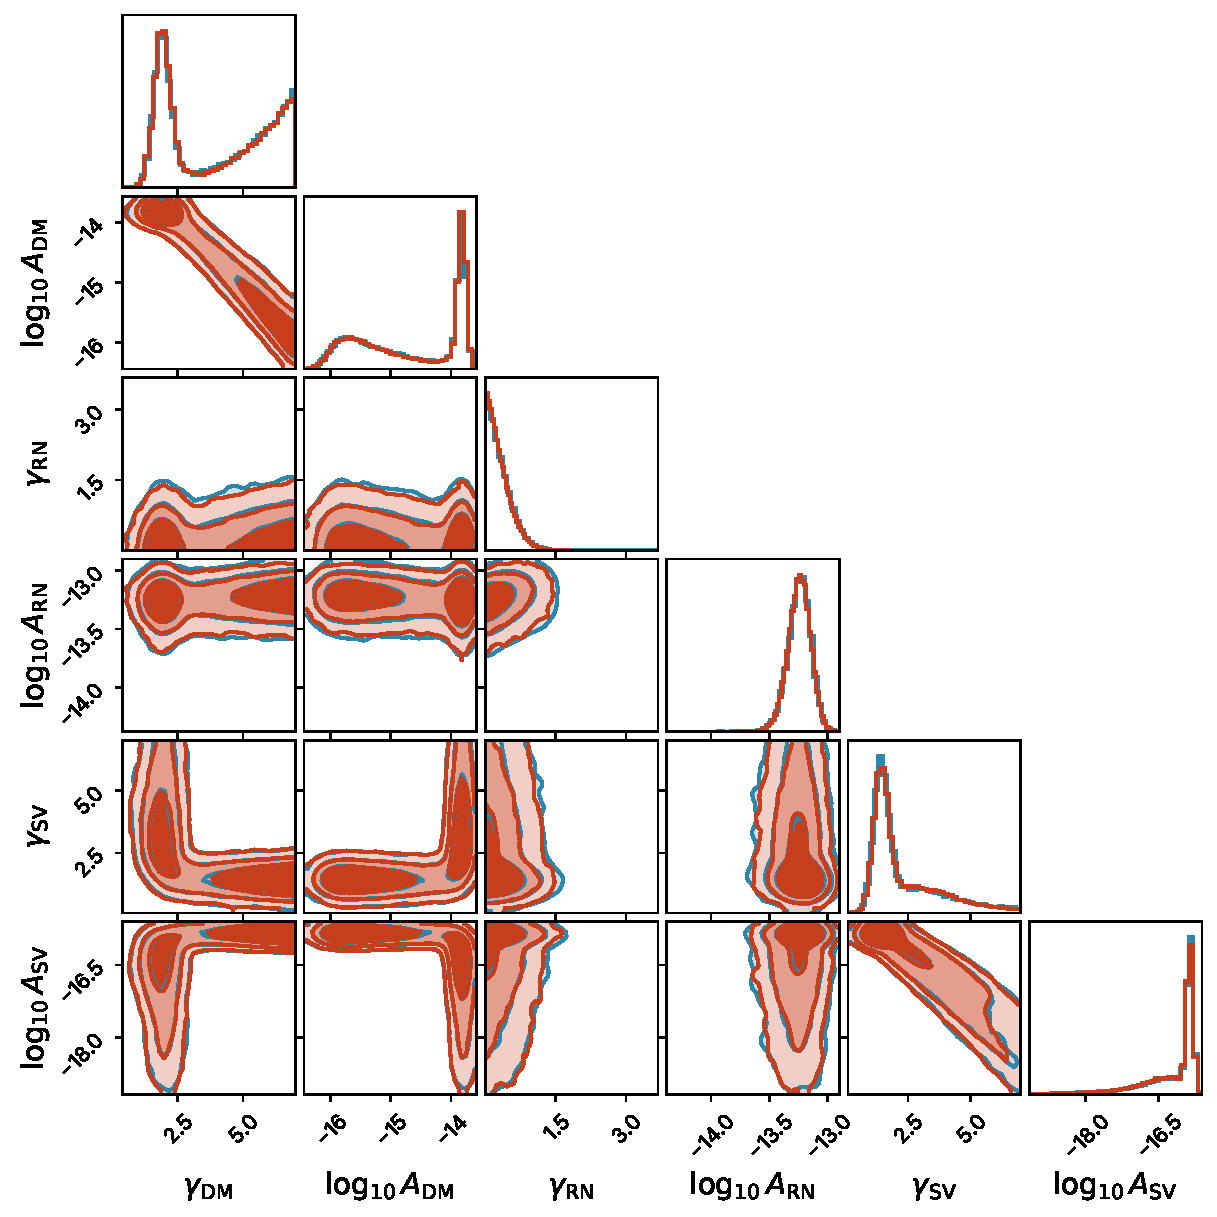
\includegraphics[height=0.82\textheight]{Figure/cap5/01_discovery_vs_enterprise.pdf}\par
  {\footnotesize \reali{Discovery} \quad \textcolor{enterprise}{Enterprise}}
\end{frame}

\begin{frame}{Riserva: GWB non modellato}
  \centering
  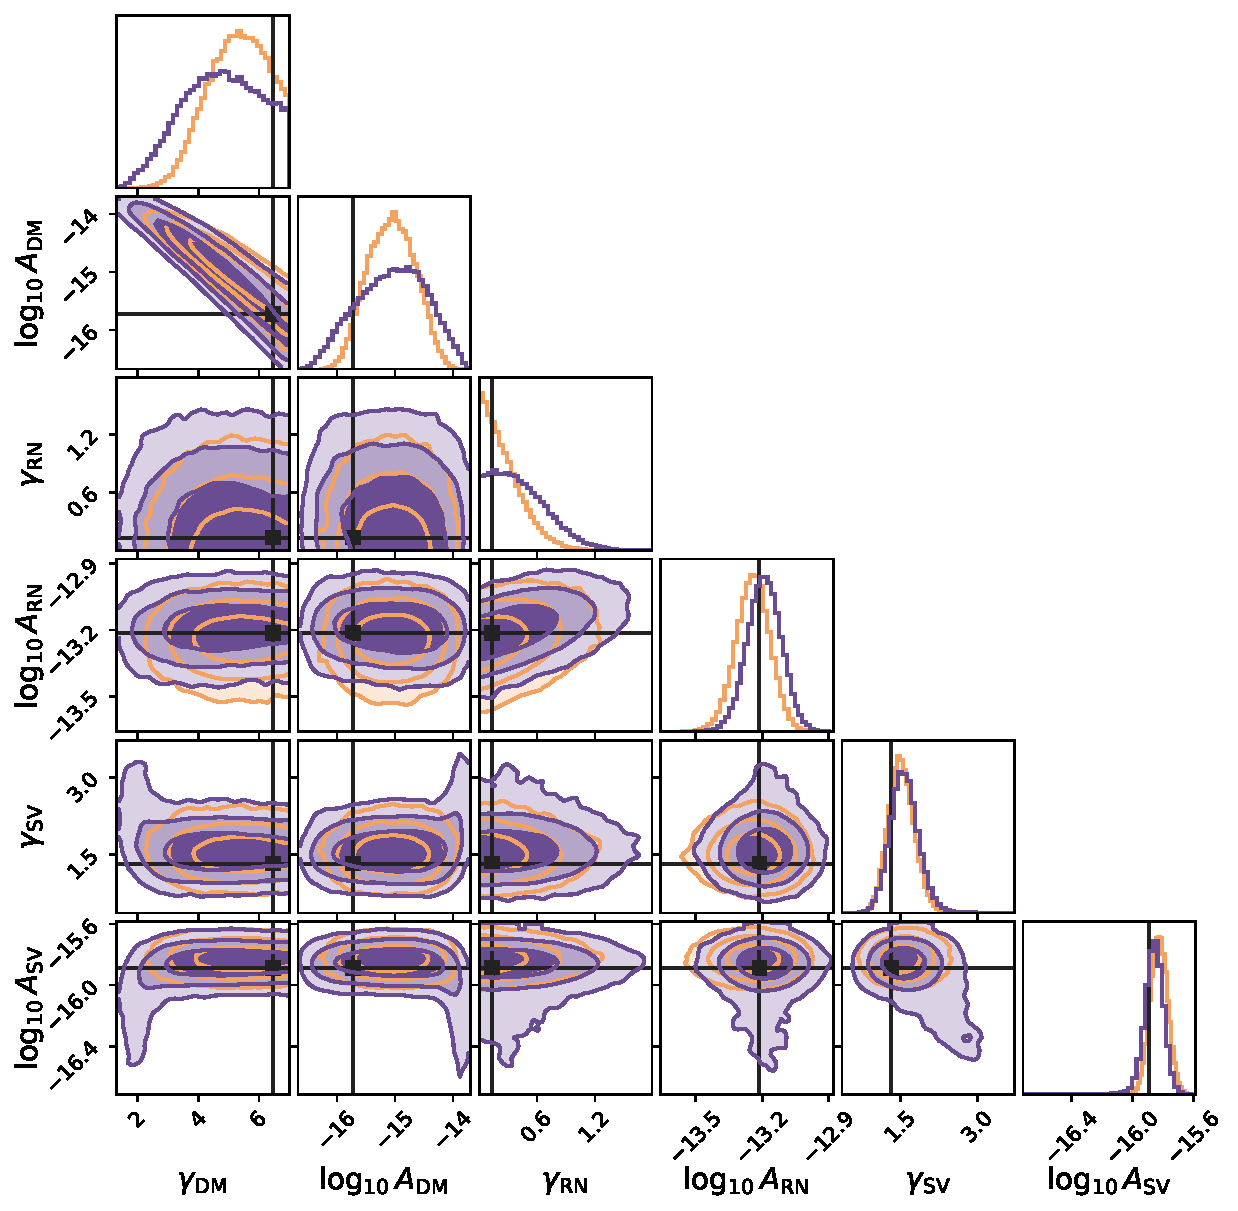
\includegraphics[height=0.82\textheight]{Figure/cap5/06_sim_noGWB_vs_gwb_A145.pdf}\par
  {\footnotesize \simul{simulazione di riferimento} \quad
   \textcolor{simdue}{con GWB, $\log_{10}\Agwb = -14.5$}}
\end{frame}

\begin{frame}{Riserva: GWB e band noise non modellati}
  \centering
  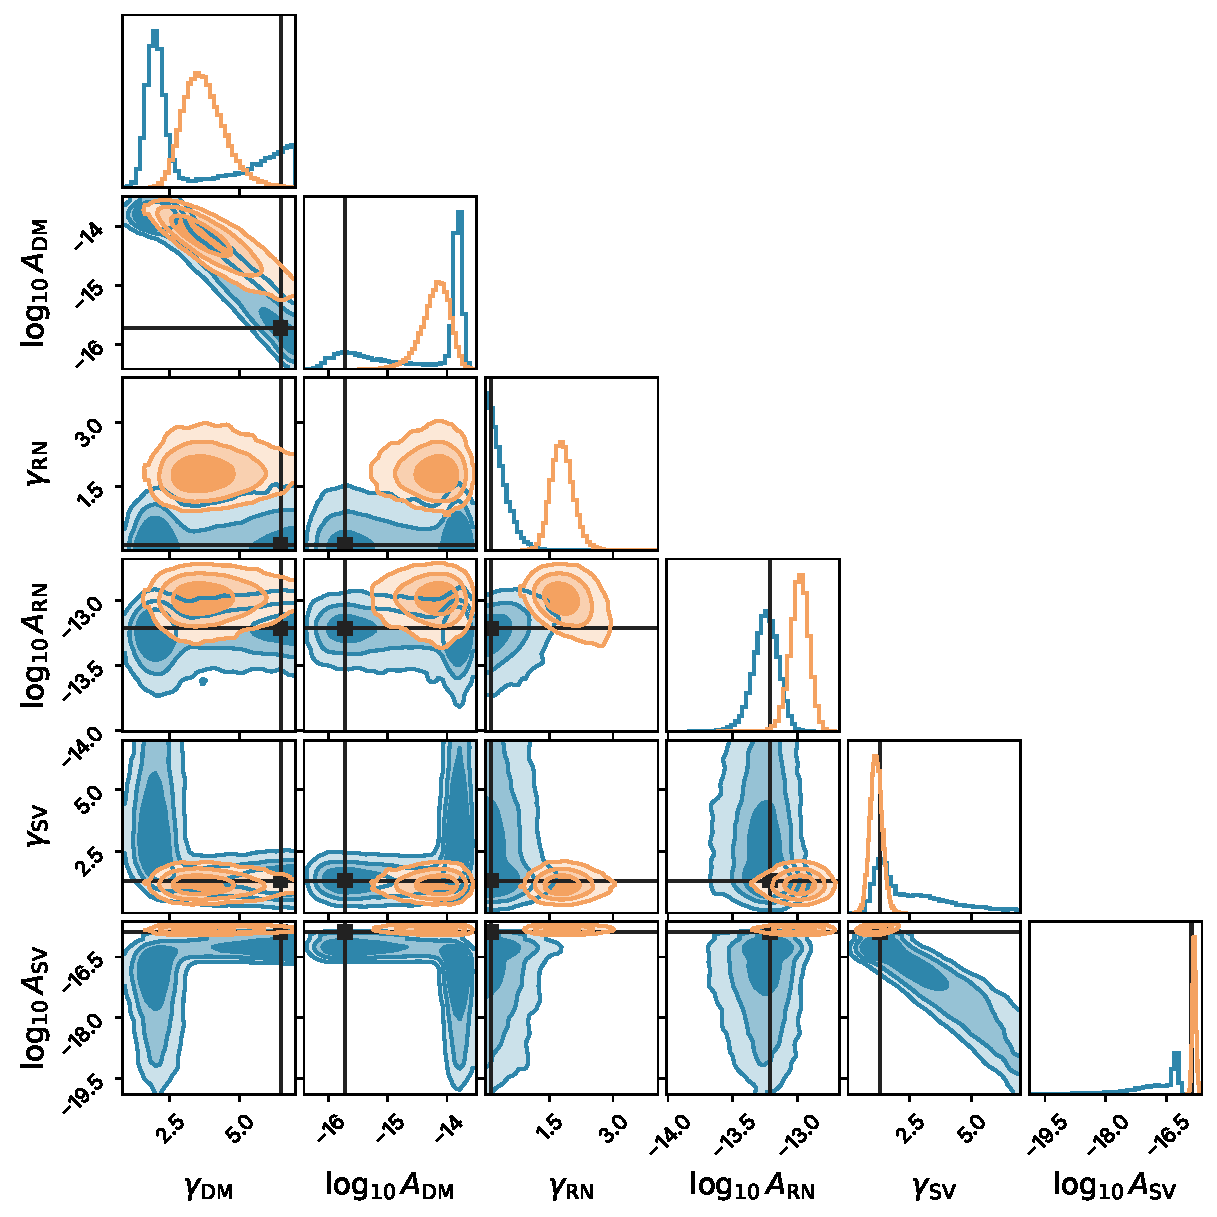
\includegraphics[height=0.82\textheight]{Figure/cap5/10_reali_vs_gwb_bn125_6par.pdf}\par
  {\footnotesize \reali{dati reali} \quad
   \simul{GWB ($-14$) + band noise ($-12.5$)}}
\end{frame}

\begin{frame}{Riserva: indice cromatico libero}
  \centering
  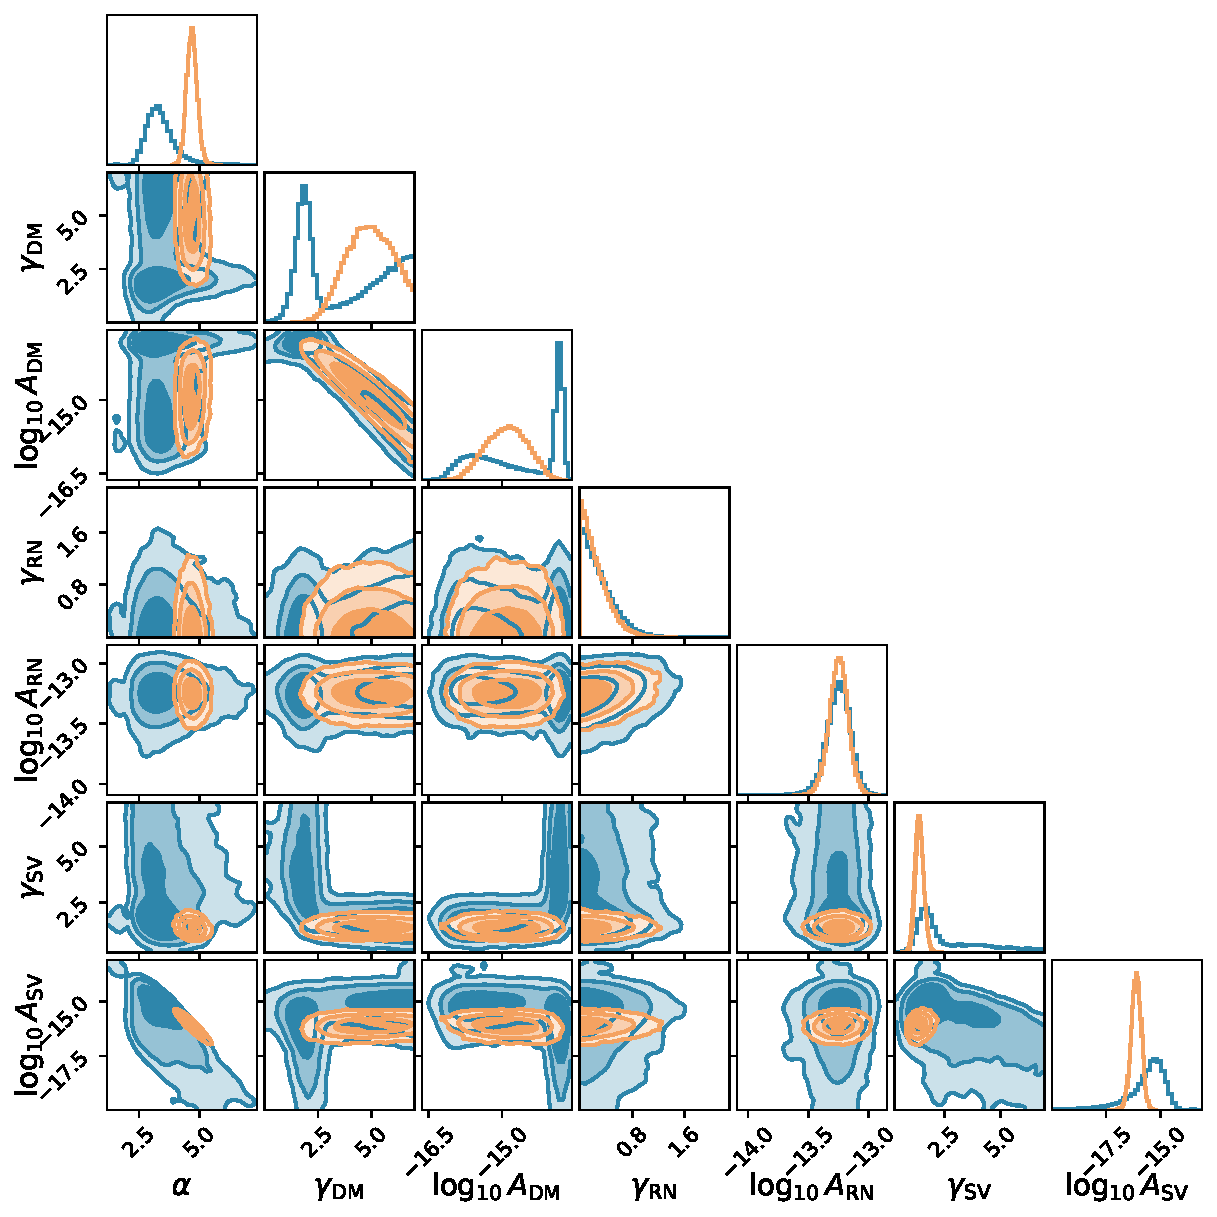
\includegraphics[height=0.82\textheight]{Figure/cap5/04_reali_vs_sim_alphafree.pdf}\par
  {\footnotesize \reali{dati reali} \quad \simul{simulazione con $\alpha = 4.4$}}
\end{frame}


\end{document}
